\section{Erwartungswert} \label{section-erwartungswert}
\index{Erwartungswert}
\subsection{Motivation}
\subsubsection{Gewinn beim Münzwurf}
Wir spielen das folgende einfache Wahrscheinlichkeitsexperiment.
In jeder Runde setzen wir einen Einsatz von einem Franken auf den
Ausgang ``Kopf'' oder ``Zahl'' des Wurfes mit einer fairen Münze.
Setzen wir richtig, erhalten wir den Einsatz zurück, zeigt die
Münze das andere Resultat, verlieren wir den Einsatz.
Die Zufallsvariable
$X(\omega)$ soll den Gewinn beim Eintreffen des Ereignisses $\omega$
angeben.

Im
langfristigen Mittel erwarten wir, dass wir in etwa der Hälfte
der Fälle gewinnen, in der anderen Hälfte verlieren.
Im Mittel
müssen wir daher davon ausgehen, dass wir pro Münzwurf einen
halben Franken gewinnen.
Der erwartete Gewinn einem einzelnen
Wurf wäre also $E(X)=0.5$.

Wir versuchen dieses Experiment zu formalisieren.
Die zugehörige
Wahrscheinlichkeitsalgebra kennt nur zwei interessante Ereignisse,
$\{\text{``Kopf''}\}$ oder $\{\text{``Zahl''}\}$.
Die Ereignisse, ihre Wahrscheinlichkeiten und wo sinnnvoll
die zu erwartenden Gewinne sind
in der Tabelle \ref{kopfzahlwahrscheinlichkeit} dargestellt.
\begin{table}
\begin{center}
\begin{tabular}{|c|c|c|}
\hline
Ereignis&Wahrscheinlichkeit&Gewinn\\
\hline
$\{\text{``Kopf''}\}$&0.5&0\\
$\{\text{``Zahl''}\}$&0.5&1\\
$\emptyset$&0&\\
$\Omega$&1&\\
\hline
\end{tabular}
\end{center}
\caption{Wahrscheinlichkeit und Gewinn bei ``Kopf oder Zahl''
\label{kopfzahlwahrscheinlichkeit}}
\end{table}
Die beiden Ereignisse $\{\text{``Kopf''}\}$ und $\{\text{``Zahl''}\}$
decken offenbar alle Möglichkeiten ab, und innerhalb des Ereignisses
ist der Gewinn einheitlich.
Der erwartete Gewinn ist also:
\[
E(\text{``Gewinn''})=\text{``Gewinn bei Kopf''}\cdot P(\text{``Kopf''})
+\text{``Gewinn bei Zahl''}\cdot P(\text{``Zahl''})
\]
Wenn etwas allgemeiner ein Spiel in $n$ verschiedene mögliche
Ausgänge (Ereignisse) $A_i$ unterteilt werden kann, die je den
Gewinn $g_i$ liefern, dann ist der erwartete Gewinn
\[
E=\sum_{i=1}^{n}g_iP(A_i).
\]

\subsubsection{Notenschnitt}
Im Beispiel des Schülers müssten wir also zunächst Ereignisse
identifizieren, und den Gewinn bestimmen, den der Schüler hat, wenn
dieses Ereignis eintritt.
Das Ereignis $A_n=\{\text{``Note $n$''}\}$
beschreibt den Fall, dass der Schüler die Note $n$ erreicht hat.
Aus den experimentellen Daten leiten wir ab, dass die Wahrscheinlichkeiten
für die einzelnen Ereignisse die folgenden sind:
\begin{align*}
P(A_1)&=0\\
P(A_2)&=0\\
P(A_3)&=\frac35\\
P(A_4)&=0\\
P(A_5)&=\frac15\\
P(A_6)&=\frac15\\
\end{align*}
Als
``Gewinn'' beim Eintreten des Ereignisses können wir die Note
ansehen, d.~h.~der Erwartungswert ist 
\[
E=\frac35\cdot 3 + \frac15\cdot 5 + \frac15\cdot 6=\frac{3\cdot 3+ 1\cdot5 + 1\cdot6}{5},
\]
also genau das, was der ``Notendurchschnitt'' auch angibt.

\subsection{Erste Definition und Rechenregeln}
Diese Beispiele führen uns auf folgende abstrakte Definition,
die in den folgenden Abschnitten konkretisiert werden soll.

\begin{definition}
Sei $X$ eine Funktion auf $\Omega$, und lasse sich $\Omega$ in endlich
viele Ereignisse $A_i$ zerlegen, auf denen $X(\omega)$ konstant ist,
dann ist der {\em Erwartungswert} von $X$
\[
E(X)=\sum_{i=0}^nP(A_i)\cdot X(A_i)
\]
\end{definition}

Der Einfachheit halber bedeutet in dieser Definition $X(A_i)$ den
konstanten Wert, den $X$ auf dem Ereignis $A_i$ annimmt.

Aus der Definition lassen sich unmittelbar folgende Rechenregeln ableiten:
\begin{satz}
\label{rechenregeln-erwartungswert}
Sind $X$ und $Y$ Zufallsvariable mit Werten in $\mathbb{R}$ ,
und $\lambda\in\mathbb{R}$, dann gilt
\begin{enumerate}
\item $E(X+Y)=E(X)+E(Y)$
\item $E(\lambda X)=\lambda E(X)$
\item Sei $\chi_A$ die charakteristische Funktion des Ereignisses $A\in{\cal A}$,
welche definiert ist durch
\[
\chi_A\colon\Omega\to\mathbb{R}:\omega\mapsto\begin{cases}
1&\omega\in A\\
0&\omega\not\in A,\\
\end{cases}
\]
dann gilt $E(\chi_A)=P(A)$.
\end{enumerate}
\end{satz}
Während die Definition ziemlich starke Einschränkungen an die Zufallsvariablen
macht, für die der Erwartungswert berechnet werden kann, können
im Satz ausgedrückten Eigenschaften die Basis für eine allgemeinere
Definition sein.
Ob nun der Erwartungswert aus der Vorstellung der Definition
entwickelt wird, oder auf Grund der Eigenschaften des Satzes konstruiert
wird, ist für die Anwendung weiter nicht wesentlich.

\subsection{Erwartungswert bei diskreten Zufallsvariablen}
In einem diskreten Wahrscheinlichkeitsraum ist es möglich, jedem
Elementarereignis eine Wahrscheinlichkeit zuzuschreiben, da die
einelementige Menge $\{\omega\}$ auch ein Ereignis ist.
Wenn man
die Elementarereignisse auch noch aufzählen kann, dann kann man
auch den Erwartungswert einfach berechnen:
\[
E(X)=\sum_{i=0}^\infty X(\omega_i)\cdot P(\{\omega_i\}).
\]
\index{Erwartungswert}
\subsubsection{Erwartete Augenzahl beim Würfeln mit einem Würfel}
Wir beschreiben des Würfeln mit einem Würfel mit Hilfe der
Elementarereignisse $\Omega=\{1,2,3,4,5,6\}$.
Offenbar handelt es sich
hier um einen diskreten Wahrscheinlichkeitsraum, in dem jedes
Elementarereignis die Wahrscheinlichkeit $\frac16$ hat.
Die Funktion
$X$ liefert die Augenzahl, also $X(i)=i$.
Die erwartete Augenzahl
ist also
\begin{align*}
E(X)&=
1\cdot\frac16+
2\cdot\frac16+
3\cdot\frac16+
4\cdot\frac16+
5\cdot\frac16+
6\cdot\frac16\\
&=\frac{1+2+3+4+5+6}6\\
&=\frac{21}{6}=3.5.
\end{align*}
\subsubsection{Erwartete Augenzahl beim Würfeln mit zwei Würfel}
Auch hier liegt ein diskreter Wahrscheinlichkeitsraum vor, dessen
Elementarereignisse die Paare $(i,j)$ sind, mit $1\le i,j\le 6$.
Die Wahrscheinlichkeit jedes einzelnen Paares ist $\frac1{36}$.
Die Funktion $X$ ist jetzt $X(i,j)=i+j$.
Der Erwartungswert ist
also
\begin{align*}
E(X)&=\sum_{i=1}^6\sum_{j=1}^6\frac{i+j}{36}
=\frac1{36}\sum_{i=1}^6\sum_{j=1}^6(i+j)
=\frac1{36}\sum_{i=1}^6\bigl(6i + \sum_{j=1}^6j\bigr)\\
&=\frac1{36}\sum_{i=1}^6(6i + 21)
%=\frac1{36}\bigl(6\sum_{i=1}^6i + 21 \bigr)
=\frac1{36}\bigl(6\sum_{i=1}^6i + 6\cdot21 \bigr)\\
&=\frac1{36}(6\cdot 21 + 6\cdot21 )
=\frac1{36}(2\cdot 6\cdot 21)
=\frac1{6}(2\cdot 21)
=7.
\end{align*}
Man kann als im Mittel mit einer Augensumme von 7 rechnen.
Dies ist
gleichzeitig auch der häufigste Wert, dies trifft aber im allgemeinen
nicht zu.

\subsubsection{Erwarteter Gewinn beim Roulette}
\index{Roulette!Gewinnerwartung}
Beim Roulette setzt man seinen Einsatz auf eine Zahl zwischen $0$
und $36$.
Gewinnt die Zahl, bekommt man das 36-fache des Einsatzes,
andernfalls erhält man nichts.
Die Wahrscheinlichkeit jeder einzelnen
Zahl ist gleich gross, nämlich $\frac1{37}$.
Der erwartete Gewinn pro
Franken Einsatz auf die Zahl $x$ ist also
\[
E(G)= \frac1{37}\cdot 36=\frac{36}{37}<1,
\]
man verliert also auf jeden Fall etwas.

Im Roulette gibt es aber weitere Spielmöglichkeiten.
Man kann zum Beispiel
auf rot setzen.
Wie gross ist der erwartete Gewinn in diesem Fall?
Im Falle einer roten Zahl gewinnt man den doppelten Einsatz,
im Falle einer schwarzen Zahl oder der Null verliert man den Einsatz.
Da eine rote Zahl mit Wahrscheinlichkeit $\frac{18}{37}$ kommt, ist
die Gewinnerwartung 
\[
E(G)=\frac{18}{37}\cdot 2=\frac{36}{37}<1.
\]
Ähnliches geschieht, wenn man vier Zahlen setzt.
Kommt eine der Zahlen,
gewinnt man das neunfache des Einsatzes, sonst ist der Einsatz 
verloren.
Die Gewinnerwartung ist wieder
\[
E(G)=\frac{4}{37}\cdot 9=\frac{36}{37}<1.
\]
Wie auch immer man es anstellt, man erhält im Mittel in jedem Spiel
weniger zurück als man eingesetzt hat.

\subsubsection{Erwarteter Gewinn beim Lotto}
\index{Lotto!Gewinnerwartung}
Beim Lotto werden $k$ Zahlen aus $N$ möglichen Zahlen gezogen.
Wenn dabei die Zahlenkombination gezogen wird, auf die man getippt
hat, gewinnt man den Hauptgewinn und den Jackpot, diesen Betrag bezeichnen
wir mit $G$.
Da die Fälle mit
weniger als sechs Richtigen nicht so viel hergeben, berechnen wir
nur den erwarteten Gewinn für sechs Richtige.

Die Ereignisalgebra für dieses Problem besteht also aus 
6-Tupeln von Zahlen, die die Lottomaschine am Wochenende ermittelt:
\[
\Omega=\{(a_1, a_2, a_3, a_4, a_5, a_6)\;|\;1\le a_i\le 45, a_i\ne a_j\}.
\]
Dabei kann natürlich niemals eine Zahl doppelt auftreten.
Das Ereignis $A$, welches den Hauptgewinn bringt, enthält alle
Elementarereignisse, die genau die Zahlen auf dem Lottozettel des
Gewinners enthalten.
Da die Lottomaschine die Zahlen in irgend einer
Reihenfolge produziert, enthält dieses Ereignis $6!$ Elementarereignisse.
Insgesamt hat $\Omega$ $N(N-1)(N-2)(N-3)(N-4)(N-5)$ Elemente, somit ist
die Wahrscheinlichkeit, dass man gewinnt:
\[
P(A)=\frac{6!}{N(N-1)(N-2)(N-3)(N-4)(N-5)}.
\]
Damit
kann man den erwarteten Gewinn ausrechnen:
\[
E(X) = P(A)\cdot G.
\]
Erst wenn dieser Betrag den Einsatz für ein einzelnes Spiel übersteigt,
ist Lottospielen rational begründbar.
Da $P(A)$ unverändert ist,
ist dazu notwendig, dass $G$ gross wird.
Da nur die Hälfte der
Einzahlungen überhaupt wieder zur Auszahlung gelangt, ist dies nur
möglich, wenn der Jackpot gross ist.
Ein grosser Jackpot zieht natürlich
auch mehr Gelegenheitsspieler an, was $G$ ebenfalls vergrössert.
\subsubsection{Niedrigere Gewinnklassen}
Natürlich
haben wir hier die niedrigeren Gewinnklassen (5 Richtige, 4 Richtige
etc.~vernachlässigt).
Um diese zu berechnen betrachten wir die folgende
Ereignisalgebra.
Elementarereignisse sind $n$-elementige Teilmengen von
$\{1,\dots,N\}$, davon gibt es $\binom{N}{n}$.
Uns interessiert das Ereignis
\[
A_k=\{\omega\;|\;|\omega\cap A|=k\},
\]
also diejenigen Elementarereignisse, die genau $k$ Elemente aus der
$M$-elementigen Teilmenge
$A\subset\Omega$ haben.
Im Beispiel des Lottos sind $A$ die Zahlen, die
auf dem Lottozettel angekreuzt sind.
Dazu müssen offenbar zunächst $k$ Zahlen aus $A$ ausgewählt werden,
und dann noch $n-k$ Zahlen aus $\Omega\setminus A$.
Ersteres ist
auf $\binom{|A|}{k}$ Arten möglich, letzteres auf $\binom{N-|A|}{n-k}$
Arten.
Insgesamt gibt es also 
\[
\binom{M}{k}\binom{N-M}{n-k}
\]
Elementarereignisse, die genau $k$ Elemnte in $A$ haben.
Insgesammt gibt es $\binom{N}{n}$.
Die Wahrscheinlichkeit,
in einem Lotto $k$ richtige
zu treffen, bei dem man auf dem Lottozettel $M$ zahlen ankreuzen kann,
und bei dem aus $N$ Zahlen $n$ gezogen werden, ist somit
\begin{equation}
h(k|N;M;n)=\frac{\binom{M}{k}\binom{N-M}{n-k}}{\binom{N}{n}}.
\label{hypergeometrische-verteilung}
\end{equation}
Dies ist die hypergeometrische Verteilung.
Mit ihr lässt sich jetzt der erwartete
Gewinn berechnen, man muss nur noch den Gewinn in jeder Klasse kennen.
Ist $G_k$ der Gewinn in der Klasse ``$k$ richtige'', dann ist der
erwartete Gewinn:
\[
E(G)=\sum_{k=0}^{6}h(k|N;M;n)G_k.
\]

\subsection{Erwartungswert und Messungen} \label{erwartungswertvonmesswerten}
\index{Erwartungswert!von Messungen}
In der Tabelle \ref{widerstandswerte} sind die Resultate der Messung des
Widerstandes zufällig eingekaufter 1k$\Omega$-Widerstände aufgeführt.
Im Kapitel 1 wurde gezeigt, dass die Mess\-werte nicht den exakten Wert
des Widerstands wiedergeben, sondern nur ein Intervall.
Eine Messung ist
also eigentlich eine Zufallsvariable, welche dem zufällig ausgewählten
Widerstand $\omega$ seinen Wert $R(\omega)$ zuordnet.
Das Messgerät zeigt
dann an, welches der Ereignisse $R^{-1}(I)$ realisiert worden ist.
Bei der Widerstandsmessung geschah dies mit folgenden Häufigkeiten:
\begin{center}
\begin{tabular}{|c|c|c|}
\hline
Ereignis&Häufigkeit&Wahrscheinlichkeit\\
\hline
$[0.989,0.990)$&6&0.30\\
$[0.990,0.991)$&7&0.35\\
$[0.991,0.992)$&5&0.25\\
$[0.982,0.993)$&2&0.10\\
\hline
\end{tabular}
\end{center}
Die Zufallsvariable $R$ hat damit folgenden Mittelwert:
\begin{align*}
E(R)&=p([0.989,0.990))\cdot 0.989+
p([0.990,0.991))\cdot 0.990\\
&\qquad  +
p([0.991,0.992))\cdot 0.991+
p([0.982,0.993))\cdot 0.992\\
&=
0.3\cdot 0.989+
0.35\cdot 0.990+
0.25\cdot 0.991+
0.1\cdot 0.992\\
&=0.99015.
\end{align*}

\subsection{Unabhängigkeit und Produktregel}
\index{Erwartungswert!Unabhängigkeit}
Für die Wahrscheinlichkeit eines Schnittereignisses $P(A\cap B)$ galt die
Produktformel
\[
P(A\cap B)=P(A)\cdot P(B)
\]
nur unter der zusätzlichen Bedingung, dass die Ereignisse $A$ und $B$
unabhängig sind.
Demzufolge ist auch für den Erwartungswert eines
Produktes $E(XY)$ zweier Zufallsvariablen zu erwarten, dass zusätzliche
Voraussetzungen gemacht werden müssen, um $E(XY)$ berechnen zu können.

\begin{figure}
\begin{center}
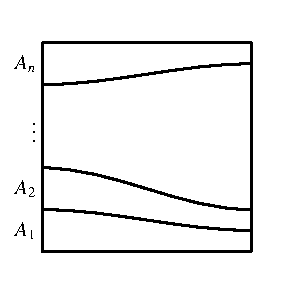
\includegraphics[width=0.3\hsize]{images/erwartung-4}
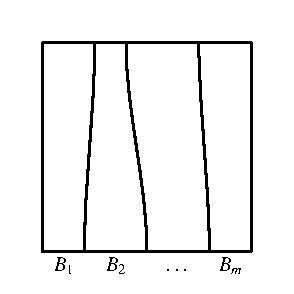
\includegraphics[width=0.3\hsize]{images/erwartung-3}
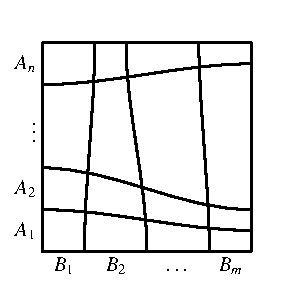
\includegraphics[width=0.3\hsize]{images/erwartung-2}
\end{center}
\caption{Ereignisse $A_i$ zur Berechnung von $E(X)$, $B_j$ zur Berechnung
von $E(Y)$ und $A_i\cap B_j$ zur Berechnung von $E(XY)$.
\label{productexpectation}}
\end{figure}
Seien $A_i$ und $B_j$ Ereignisse so, dass $X$ auf den $A_i$ und $Y$ auf
den $B_j$ konstant ist.
Dann kann man die Ereignisse $A_i\cap B_j$
zur Berechnung des Erwartungswertes heranziehen, wie in
Abbildung~\ref{productexpectation}, denn auf ihnen ist sowohl $X$ wie
auch $Y$ konstant.
Die Wahrscheinlichkeit von $A_i\cap B_j$ kann aber nur dann
durch die Wahrscheinlichkeiten von $A_i$ und $B_j$ ausgedrückt werden,
wenn die Ereignisse $A_i$ und $B_j$ paarweise
unabhängig sind.
Dann berechnet man:
\begin{align*}
E(XY)&=\sum_{i=1}^n\sum_{j=1}^m X(A_i\cap B_j)Y(A_i\cap B_j)P(A_i\cap B_j)\\
&=\sum_{i=1}^n\sum_{j=1}^m X(A_i)Y(B_j)P(A_i)P(B_j)\\
&=\sum_{i=1}^n X(A_i)P(A_i)\sum_{j=1}^mY(B_j)P(B_j)\\
&=E(X)\cdot E(Y).
\end{align*}
Die oben verwendete Unabhängigkeitsbedingung kann man mit folgender
Definition erzwingen:
\begin{definition}Zwei Zufallsvariable $X$ und $Y$ heissen
unabhängig, wenn die Ereignisse $\{\omega|X(\omega)\le x\}$
und $\{\omega|Y(\omega)\le y\}$ für alle $x,y\in\mathbb R$
unabhängig sind, also
\[
P((X\le x)\wedge(Y\le y))=P(X\le x)\,P(Y\le y)\quad\forall x,y\in\mathbb{R}.
\]
\end{definition}
\index{Produktregel!für den Erwartungswert}
Damit haben wir auch für Zufallsvariable eine Produktregel:
\begin{satz}
\label{produktregel-erwartungswert}
Sind $X$ und $Y$ unabhängige Zufallsvariablen, dann gilt
\[
E(XY)=E(X)\cdot E(Y).
\]
Für zwei beliebige Funktionen $f$ und $g$ von $\mathbb{R}$ nach $\mathbb{R}$,
so dass $f(X)$ und $g(Y)$ immer noch Zufallsvariable sind, gilt
\[
E(f(X)g(Y))=E(f(X))E(g(Y)).
\]
\end{satz}
Seien $X$ und $Y$ die Augenzahlen beim Würfeln mit zwei Würfeln.
Die Ereignisse $X\le x$ und $Y\le y$ sind offensichtlich unabhängig
(``horizontale und vertikale Streifen''), daher gilt
\[
E(XY)=E(X)E(Y)=3.5^2=12.25.
\]

\subsection{Erwartungswert und Integration}
\index{Erwartungswert!und Integration}
Die Berechnung des Erwartungswertes war im vorangegangene Abschnitt
einfach möglich, weil wir annehmen konnten, dass es Ereignisse $A$
gibt, auf denen die Zufallsvariable $X$ konstant ist.
Wenn diese
Bedingung nicht mehr gilt, könnte man versuchen, den Erwartungswert
durch die Summe der kleinsten und grössten möglichen Werte auf jedem
Ereignis $A_i$ einzuschachteln:
\[
\sum_{i=0}^nP(A_i)\min_{\omega\in A_i}X(\omega)
\le E(X)\le
\sum_{i=0}^nP(A_i)\max_{\omega\in A_i}X(\omega).
\]
Wir betrachten als Spezialfall die Ereignisalgebra für eine
Messung, hier ist $\Omega=\mathbb{R}$.
Die Wahrscheinlichkeitsfunktion $P$
liefert zu jedem Teilintervall $I\subset \mathbb{R}$ eine Wahrscheinlichkeit.
Wir betrachten eine Zerlegung der reellen Achse in Teilintervalle $I_i$.
Zu einer Funktion $X\colon \mathbb{R}\to\mathbb{R}$ kann man jetzt den
Erwartungswert wie folgt berechnen:
\[
\sum_{i=0}^nP(I_i)\min_{x\in I_i}X(x)
\le E(X)\le
\sum_{i=0}^nP(I_i)\max_{x\in I_i}X(x).
\]
Diese Konstruktion ist aber aus der Analysis vertraut, auf diese
Art wurde das Integral konstruiert.
Die Summenausdrücke sind sogenannte
Riemannsche Summen, der einzige Unterschied ist, dass nicht die Länge des
Intervalls, sondern die Wahrscheinlichkeit $P(I_i)$ des Intervalls gemessen
wird.
Der Erwartungswert ist also eine Art verallgemeinertes Integral,
wofür der Mathematiker auch 
\[
E(X)=\int_{\Omega}X(\omega)dP(\omega)
\]
schreibt.
Da uns diese Betrachtungsweise keine wirklich praktikablen
Möglichkeiten zur Berechnung von $E(X)$ bietet, verfolgen wir sie
hier nicht weiter, werden aber im nächsten Kapitel eine verwandte
Technik kennen lernen, welche nur gewöhnliche Integrale verwendet.

